\section{Spatial data formats and storage models}
\label{sec:spatial-data-formats}

Spatial data storage spans a spectrum from simple flat files to full database engines. At one end, a format may be a self-contained file that any application can read directly from disk, and at the other, the data lives inside a server process that mediates all access through a query language. Between these two sit single-file databases that bundle an embedded engine into a portable file. The choice of tier shapes, which access patterns are efficient, how data scales, and whether the format fits the decoupled storage and compute model of cloud architectures \parencite{cngfoundation2024_cloud_optimized_geospatial_formats_guide}. This section presents the three tiers in turn: flat file formats, file databases, and full database engines. Each subsection first defines the concept and then describes the concrete implementations relevant to this thesis.

\subsection{File formats}
\label{sec:file-formats}
A file format in this context is a self-contained file or bundle of files that encodes spatial data without an accompanying engine. An external library that knows the format is often required to read the data. Typically, the data is read sequentially or via random access at byte offsets. Object storage in cloud environments differs fundamentally from local disk access, as each read operation is an HTTP request carrying per-request latency on the order of tens of milliseconds. This overhead makes patterns that issue many small requests inefficient \parencite{esri2024_cloud_imagery_storage}. Cloud-native file formats address this by structuring the file so that a client can retrieve only the byte ranges it needs through HTTP range requests, using internal metadata to locate the relevant chunks of data without downloading the entire file \parencite{ogc2023_cog_standard_21026}.

\subsubsection{Shapefile}
The Shapefile is a vector data format introduced by \acrfull{esri} in 1998 and remains one of the most widely supported formats in the \acrshort{gis} ecosystem \parencite{esri1998_shapefile_technical_description}. A Shapefile is not a single file but a bundle of files sharing a common prefix, with three mandatory files and several optional ones. The components are listed in Table~\ref{tab:shapefile-components}.

\begin{table}[H]
    \centering
    \begin{tabular}{lll}
        \toprule
        \textbf{Extension} & \textbf{Type} & \textbf{Content} \\
        \midrule
        \texttt{.shp} & Mandatory & Variable-length geometry records \\
        \texttt{.shx} & Mandatory & Byte offsets into main file \\
        \texttt{.dbf} & Mandatory & Feature attributes (dBASE table) \\
        \texttt{.prj} & Optional & \acrlong{crs} (\acrshort{wkt}) \\
        \texttt{.sbn} / \texttt{.sbx} & Optional & Spatial index (\acrshort{esri}, undocumented) \\
        \texttt{.qix} & Optional & Spatial index (quadtree, open-source) \\
        \bottomrule
    \end{tabular}
    \caption[Shapefile component files.]{Mandatory and optional files in the Shapefile format.}
    \label{tab:shapefile-components}
\end{table}

The three mandatory files are tightly coupled by record order. A record is the storage unit for one feature, holding the geometry in the \texttt{.shp} file and the corresponding attribute values in the \texttt{.dbf} file. The \texttt{.shp} file begins with a 100-byte header followed by a sequence of variable-length records, each prefixed by an 8-byte record header that contains the record number and the content length of the record \parencite{esri1998_shapefile_technical_description}. Because records vary in length, finding the \(n\)th record by reading the \texttt{.shp} file alone would require scanning every preceding record. The \texttt{.shx} file solves this by storing a fixed-length 8-byte entry per record that gives the byte offset and length of the corresponding record in the \texttt{.shp} file, which allows a reader to jump directly to any record by number \parencite{esri1998_shapefile_technical_description}. The \texttt{.dbf} file holds one attribute row per geometry in the same order as the \texttt{.shp} file, so attributes and geometries are joined by position rather than by a key column \parencite{esri1998_shapefile_technical_description}.

A Shapefile is restricted to a single geometry type per file, chosen from fourteen possible values that include 2D, 3D and measured variants of points, polylines, polygons and multipoints \parencite{esri1998_shapefile_technical_description}. The format does not record topology and does not define a \acrfull{crs} in the original specification; \acrshort{crs} information is supplied through an auxiliary \acrfull{wkt} file that emerged as a de facto convention with later \acrshort{esri} products \parencite{esri1998_shapefile_technical_description, gdal2025_shapefile_driver}.

The \texttt{.shx} index provides direct access to any feature record by byte offset, but it is a record index rather than a spatial index. It cannot increase the query speed of bounding-box or intersection queries. A spatial index must be created separately and stored in one of the auxiliary files in Table~\ref{tab:shapefile-components}, either \acrshort{esri} 's undocumented \texttt{.sbn}/\texttt{.sbx} files or the quadtree \texttt{.qix} files used by MapServer and \acrfull{gdal} \parencite{gdal2025_shapefile_driver}. Without such an index, evaluating a spatial predicate requires a sequential scan of the \texttt{.shp} file, reading and parsing every record in order, since the format carries no per-record or per-block metadata that would let a reader skip features without first reading them.

The format also imposes strict size limits. The file length field in the \texttt{.shp} and \texttt{.dbf} files is a 32-bit signed integer measured in 16-bit words \parencite{esri1998_shapefile_technical_description}, which mathematically caps each of these component files at 2~GB \parencite{wikipedia2025_esri_shapefile, gdal2025_shapefile_driver}. Datasets that exceed this size must be partitioned across multiple Shapefiles. Floating-point values are stored as text rather than binary, which can introduce rounding errors on read and write \parencite{esri2024_arcmap_shapefile_output}, and the format has no native representation of \texttt{null}, with \acrshort{esri} software writing null values as zero \parencite{wikipedia2025_esri_shapefile}.

\subsubsection{GeoJSON}
GeoJSON is a text-based format for geographic data based on \acrfull{json}. It was standardized as \acrshort{ietf} \acrshort{rfc}~7946 in August 2016, replacing a 2008 community specification \parencite{butler2016_rfc7946_geojson_format}. Its \acrfull{iana} media type is \texttt{application/geo+json}, with file extensions \texttt{.json} or \texttt{.geojson} \parencite{butler2016_rfc7946_geojson_format}.

A GeoJSON document is a single \acrshort{json} object of one of nine types, listed in Table~\ref{tab:geojson-types}. Seven are geometry types from the \acrfull{ogc} Simple Features standard. The other two, Feature and FeatureCollection, are unique to GeoJSON and attach attributes to geometries \parencite{butler2016_rfc7946_geojson_format}. A Feature combines a geometry with a \acrshort{json} \texttt{properties} object holding its attributes. A FeatureCollection is a list of Features. Unlike Shapefile's \texttt{.shp}/\texttt{.dbf} pairing, geometries, and attributes are stored together, so a reader always parses them as a single unit.

\begin{table}[H]
    \centering
    \begin{tabular}{ll}
        \toprule
        \textbf{Type} & \textbf{Category} \\
        \midrule
        Point               & Geometry \\
        MultiPoint          & Geometry \\
        LineString          & Geometry \\
        MultiLineString     & Geometry \\
        Polygon             & Geometry \\
        MultiPolygon        & Geometry \\
        GeometryCollection  & Geometry \\
        Feature             & Wrapper  \\
        FeatureCollection   & Wrapper  \\
        \bottomrule
    \end{tabular}
    \caption[GeoJSON top-level types.]{The nine top-level types defined by the GeoJSON specification.}
    \label{tab:geojson-types}
\end{table}

Coordinates are \acrshort{json} arrays of two or three numbers: longitude, latitude, and optional altitude. Implementations should not use more than three elements \parencite{butler2016_rfc7946_geojson_format}. \acrshort{rfc}~7946 requires all coordinates to be in WGS84 longitude and latitude (\texttt{OGC:CRS84}), removing support for alternative reference systems that caused interoperability problems \parencite{butler2016_rfc7946_geojson_format}. The standard also mandates the right-hand rule for polygon rings (exterior counterclockwise, holes clockwise) and uses \texttt{[west, south, east, north]} for bounding boxes instead of \texttt{minx, miny, maxx, maxy} \parencite{butler2016_rfc7946_geojson_format}.

GeoJSON has no indexing mechanism. Unlike Shapefile's \texttt{.shx}, it lacks structures for fast access, row-group statistics, or embedded metadata to identify byte ranges. To evaluate any query, spatial or attribute-based, every Feature must be parsed from the start of the file. Because it uses \acrshort{json}, a parser cannot skip Features; it must read and tokenize all contents. The \texttt{type} field might appear only after a massive \texttt{features} array, so large files must be read completely before confirming their structure \parencite{butler2016_rfc7946_geojson_format}.

GeoJSON is plain text, readable by any tool supporting \acrshort{json}. This makes it popular for web maps, \acrshort{json}-based \acrshort{api}s, and ad hoc data exchange. However, at scale, these features become limitations. Files cannot be partially parsed, so the entire document must be downloaded before use, making it unsuitable for cloud-optimized access \parencite{cngfoundation2024_cloud_optimized_geospatial_formats_guide}. Higher coordinate precision can greatly increase file size; raising precision from six to fifteen decimal places can nearly double the size of files with many detailed polygons \parencite{butler2016_rfc7946_geojson_format}.

\subsubsection{Geography Markup Language}
\acrfull{gml} is an \acrshort{xml}-based format for geographic information, standardized as \acrshort{ogc} 07-036 and ISO 19136:2007 \parencite{ogc2007_07036_gml_specification}. Version 3.2.1 is the main reference. A \acrshort{gml} dataset has two parts: an \acrshort{xml} Schema (\texttt{.xsd}) describing the application schema, and an \acrshort{xml} instance document containing feature data \parencite{ogc2007_07036_gml_specification}. The meaning of any feature depends on its schema, not just the document. Application schemas such as CityGML (3D city models) and AIXM (aviation data) extend the base \acrshort{gml} schema with domain-specific types. To interpret an instance, a reader needs access to the relevant schema \parencite{wikipedia2026_geography_markup_language}.

\acrshort{gml}'s geometry model is richer than Simple Features. Besides basic primitives, it supports non-linear curves such as arcs and splines, composite geometries, solids, and topology primitives for shared edges and nodes \parencite{ogc2007_07036_gml_specification}. Each geometry includes its coordinate reference system via an \texttt{srsName} attribute, usually referencing an \acrshort{ogc} \acrshort{uri} like \texttt{urn:ogc:def:crs:EPSG::4326}. The axis order follows the referenced \acrshort{crs}; for EPSG:4326, this means latitude before longitude, unlike GeoJSON \parencite{gdal2025_gml_driver}.

\acrshort{gml} has no native indexing scheme of its own and relies on existing indexing techniques applied at the database level \parencite{lu2005_advances_in_gml_geospatial_applications}. Parsing is either incremental with a \acrshort{sax} parser, which uses low memory and is well-suited to point and range queries. Still, it becomes inefficient when queries involve many attributes, or full with a \acrshort{dom} parser, which offers richer query flexibility at substantially higher memory cost \parencite{lu2005_advances_in_gml_geospatial_applications}. Neither lets a reader skip features without tokenizing the surrounding \acrshort{xml}, and there is no structural counterpart to Shapefile's \texttt{.shx} or to row-group statistics. Any query, therefore, requires reading and parsing the relevant part of the document in full.

\acrshort{gml} 's main drawback is verbosity. Documents are large due to frequent repeated \acrshort{xml} tags, attribute names, and high-precision coordinates stored as text \parencite{guo2010_effective_gml_documents_compressor}. The lack of native indexing combined with the parsing overhead makes large datasets impractical to query in place, so they are often loaded into spatial databases for analysis \parencite{li2004_gml_storage_spatial_database}. Because instance documents cannot be interpreted without their accompanying schema, \acrshort{gml} is also less self-contained than formats like GeoJSON or Shapefile, which complicates ad hoc data exchange.

Despite these drawbacks, \acrshort{gml} remains the default encoding in the European public-sector spatial data infrastructure. The INSPIRE Directive 2007/2/EC is implemented through Commission Regulation (EU) No 1089/2010, and the INSPIRE Guidelines for the Encoding of Spatial Data set \acrshort{gml} (\acrshort{iso} 19136) as the default encoding used by most INSPIRE data specifications \parencite{inspire2023_d27_encoding_guidelines, ec2010_commission_regulation_1089_inspire}.

\subsubsection{GeoParquet}
GeoParquet is a cloud-native vector format for storing geospatial data in Apache Parquet, a columnar file format built for analytical workloads on distributed systems \parencite{ogc2024_geoparquet_specification_v110, lamb2022_querying_parquet_millisecond_latency}. Its cloud-native nature stems from the Parquet format itself, not from any geospatial feature, and it reflects the shift from row-oriented to columnar storage in modern data platforms.

GeoParquet files follow Parquet's internal structure, illustrated in Figure~\ref{fig:geoparquet-file-format}. Rows are organized into row groups, which are contiguous, independently readable partitions. Within each group, data is stored column-wise, keeping each attribute's values together. The file footer contains a metadata index with the location and min/max values for every column in each row group \parencite{lamb2022_querying_parquet_millisecond_latency}. Geometry columns are stored as Parquet \texttt{BYTE\_ARRAY}, encoded in \acrfull{wkb} or GeoArrow, so per-group statistics also apply to geometry \parencite{ogc2024_geoparquet_specification_v110}.

\begin{figure}[H]
    \centering
    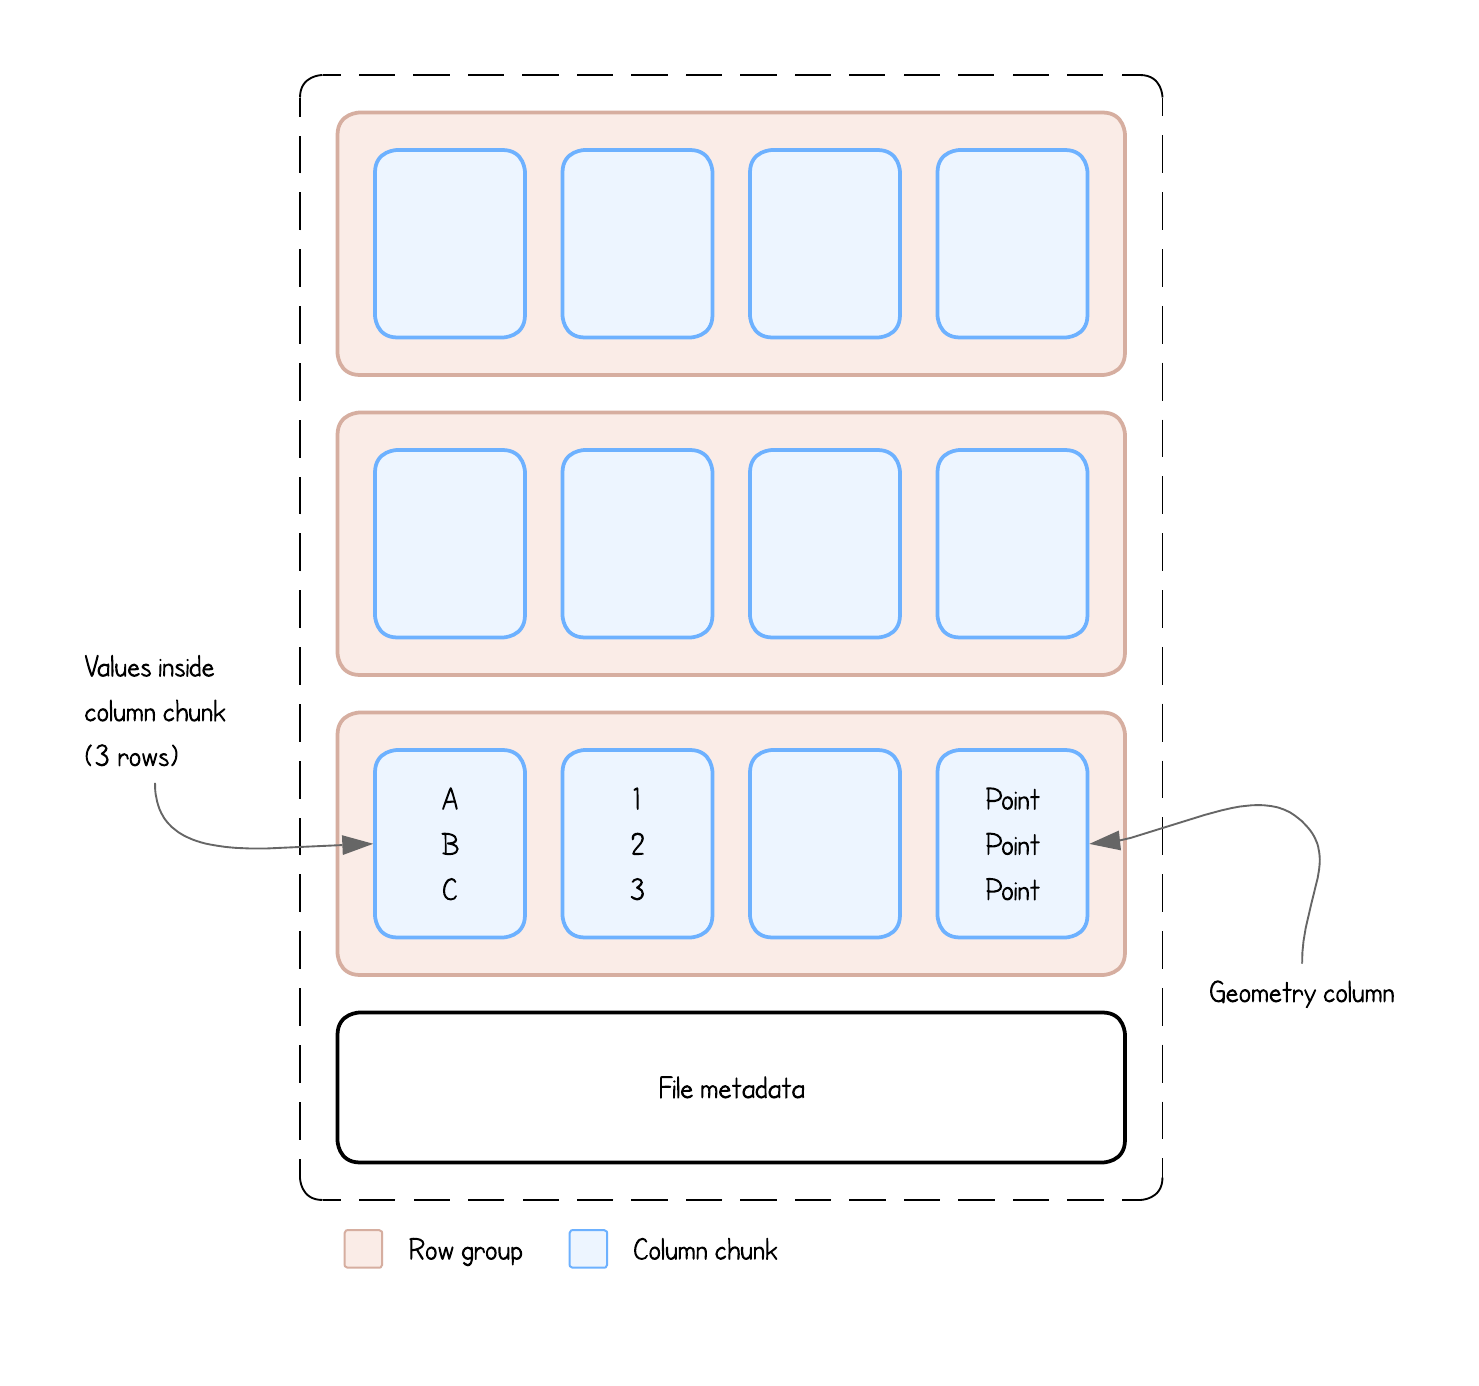
\includegraphics[width=0.8\textwidth]{Chapters/02-background/sub-chapters/figures/02-geoparquet-file-format.png}
    \caption[Internal structure of a GeoParquet file.]{Internal structure of a GeoParquet file. Rows are grouped into row groups, each holding one column chunk per column, and the file footer holds the metadata index with location and min/max statistics for every column chunk.}
    \label{fig:geoparquet-file-format}
\end{figure}

Coordinate reference systems are described in PROJJSON, a JSON encoding of WKT2:2019. If not specified, the default CRS is \texttt{OGC:CRS84} (WGS84 longitude and latitude) \parencite{ogc2024_geoparquet_specification_v110}. GeoParquet enforces \texttt{(x, y)} axis order, overriding the CRS and avoiding latitude/longitude confusion found in formats like \acrshort{gml} \parencite{ogc2024_geoparquet_specification_v110}.

The file format is built for selective reads. The footer index lets a query engine compare predicates against each row group's min and max statistics, skipping groups that cannot match, an optimization called predicate pushdown \parencite{lamb2022_querying_parquet_millisecond_latency}. The columnar format also enables projection pushdown, so only needed columns are read \parencite{lamb2022_querying_parquet_millisecond_latency}. GeoParquet 1.1 adds spatial filters using an optional bounding-box encoding that stores per-row \texttt{xmin}, \texttt{ymin}, \texttt{xmax}, \texttt{ymax} columns, allowing spatial queries to benefit from the same pruning as scalar filters \parencite{ogc2024_geoparquet_specification_v110}. Though Parquet was built for \acrfull{hdfs}, its access pattern also fits commodity object storage because both have similar characteristics \parencite{lamb2022_querying_parquet_millisecond_latency}. Readers use \acrshort{http} range requests to retrieve the footer and needed row groups, skipping the rest \parencite{cngfoundation2024_cloud_optimized_geospatial_formats_guide}.

Its main limitations stem from its static columnar design. Parquet files are immutable, so any update or append requires rewriting the entire file \parencite{microsoft2024_direct_lake_parquet_immutability}. Many small files also perform poorly, as each must fetch its footer on open \parencite{cngfoundation2024_geoparquet_guide}. Spatial indices are not included. The 1.1 bbox covering allows row-group pruning but cannot replace a true R-tree for complex joins or nearest-neighbor searches \parencite{cngfoundation2024_geoparquet_guide}. The geometry model is more limited than some alternatives, lacking support for M values, non-linear geometry types, and requiring geometry columns at the schema root \parencite{ogc2024_geoparquet_specification_v110}. For best results, the specification suggests row groups of 50,000--150,000 rows, spatial partitioning for files over 2~GB, and zstd compression \parencite{ogc2024_distributing_geoparquet}.

\subsubsection{Mapbox Vector Tiles}
\acrfull{mvt} is a compact encoding for tiled vector data, built for fast browser or server-side rendering \parencite{mapbox2017_vector_tile_specification_21}. At version 2.1, it is not a formal \acrshort{ogc} standard. Still, it is defined as a tile encoding class in the \acrshort{ogc} \acrshort{api} -- Tiles standard (\acrshort{ogc} 20-057) \parencite{ogc2022_20057_api_tiles} and included in the GeoPackage Vector Tiles Extension \parencite{ogc2018_vector_tiles_pilot_geopackage_extension}. A tile server typically serves tiles via URLs such as \texttt{/z/x/y.mvt}.

An \acrshort{mvt} tile uses Google Protocol Buffers as its serialization format \parencite{mapbox2017_vector_tile_specification_21}. Each tile contains one or more named layers, and each layer holds features whose geometry is encoded as a sequence of 32-bit unsigned integer commands (MoveTo, LineTo, ClosePath) operating in tile-local coordinates \parencite{mapbox2017_vector_tile_specification_21}. Attributes are encoded as integer pairs that index into per-layer keys and values arrays, which deduplicates repeated strings and reduces tile size \parencite{mapbox2017_vector_tile_specification_21}. The default tile extent is 4096 units, and geometries may extend beyond it to act as a rendering buffer for clean edges between adjacent tiles \parencite{mapbox2017_vector_tile_specification_21}.

\acrshort{mvt} supports four geometry types (UNKNOWN, POINT, LINESTRING, POLYGON), with no collection type, and the y-axis points downward in tile-local coordinates \parencite{mapbox2017_vector_tile_specification_21}. A tile does not contain its own bounds or projection; the decoder is assumed to know these from context, with Web Mercator and the Google tile scheme as the conventional defaults \parencite{mapbox2017_vector_tile_specification_21}.

The \acrshort{mvt} specification is narrowly scoped and does not define how tiles are stored, requested, or shared \parencite{mapbox2017_vector_tile_specification_21}. The access model is the tile pyramid: clients request only the tiles that cover their viewport at the current zoom level, and spatial filtering occurs via \acrshort{url}s, not within tiles.

\acrshort{mvt} has several limitations that follow from its rendering-first design. The format has no internal indexing, and there is no way to query individual features without fully decoding the tile. Coordinates are quantized to the tile's integer grid, which loses precision and prevents reverse engineering of exact source coordinates \parencite{mapbox2017_vector_tile_specification_21}. The specification leaves encoding of attribute arrays or nested objects up to the encoder, limiting fidelity for complex schemas \parencite{mapbox2017_vector_tile_specification_21}. Tiles are also usually pre-generated for a specific tile scheme and zoom range, so changes to source data require regenerating the relevant tiles.

\subsubsection{PMTiles}
While \acrshort{mvt} defines a single tile's contents, PMTiles packages and delivers multiple tiles as a single cloud-native archive. PMTiles version 3 is a single-file archive format for an entire tile pyramid, allowing direct retrieval from object storage using \acrshort{http} range requests \parencite{protomaps2024_pmtiles_specification_v3, cngfoundation2024_pmtiles_guide}. The format supports cloud-native delivery without a tile server; the client reads the archive directly \parencite{cngfoundation2024_pmtiles_guide}. Tiles in a PMTiles archive can be \acrshort{mvt}, PNG, JPEG, WebP, or AVIF. \acrshort{mvt} is typically used for vector basemaps \parencite{protomaps2024_pmtiles_specification_v3}.

A PMTiles archive has a fixed layout of header, root directory, metadata, leaf directories, and tile data \parencite{protomaps2024_pmtiles_specification_v3}. The root directory must fit within the first 16~KiB so that latency-sensitive clients can fetch it in a single initial request \parencite{protomaps2024_pmtiles_specification_v3}. The two-level directory allows any tile to be retrieved with at most two more \acrshort{http} requests after the root \parencite{protomaps2023_pmtiles_v3_whats_new}.

Tiles are referenced by a TileID based on Hilbert curve order, so spatially adjacent tiles get similar identifiers \parencite{protomaps2024_pmtiles_specification_v3, cngfoundation2024_pmtiles_guide}. This supports run-length encoding of repeated tiles and request batching when the archive uses clustered Hilbert order \parencite{protomaps2024_pmtiles_specification_v3, protomaps2023_pmtiles_v3_whats_new}. PMTiles is typically used with the Web Mercator grid, following the same convention as \acrshort{mvt} \parencite{cngfoundation2024_pmtiles_guide}.

The directory structure is a hierarchical index over the tile pyramid. Given a Z/X/Y coordinate, the client converts it to a TileID, locates the entry via the root and leaf directories, and issues a range request for the corresponding byte range within the tile data section. There is no sequential scan or server-side computation, and unrequested tiles are not transferred.

PMTiles is read-only and shares the same static-file constraints as formats like Parquet. Archives cannot be updated in place; any change requires rewriting the entire file, and transactional updates require falling back to a database \parencite{protomaps2024_pmtiles_concepts}. The single-file design also prevents parallel writes. The format inherits the limitations of its embedded tiles; for vector tiles, this includes the rendering-oriented constraints of \acrshort{mvt} described above. The 16~KiB root-directory cap trades off against archive size, as larger or deeper pyramids push more of the directory structure into leaf directories, increasing the chance that a tile lookup needs a second request \parencite{protomaps2024_pmtiles_specification_v3, protomaps2023_pmtiles_v3_whats_new}.

The file formats above differ along one key axis: whether a client can read part of a file without parsing it entirely. Shapefile, GeoJSON, and \acrshort{gml} require a full scan for any query, which makes them a poor fit for object storage. GeoParquet and PMTiles expose internal metadata, allowing a client to request only the byte ranges it needs via \acrshort{http} range requests. \acrshort{mvt} falls outside this split, since it encodes a single tile rather than a full dataset. This divide between full-scan and range-request formats is the primary axis for interpreting the benchmarking results in Section~\ref{ch:discussion}.

\subsection{File databases}
\label{sec:file-databases}
A file database is a single, portable file that contains data, an embedded query engine, and indexes. Unlike a flat file, it can answer queries using its own indexes. Unlike a server-based engine, it does not need a separate process. The engine is part of the application and accesses the file through standard function calls. This makes file databases easy to deploy and move between machines. However, relying on file-level coordination instead of a server process limits write concurrency. File databases work well for single-user analysis and data exchange, but not for workloads with many concurrent writes. The following subsections describe three geospatial file databases: SQLite with SpatiaLite, the \acrshort{esri} File Geodatabase, and OGC GeoPackage.

\subsubsection{SQLite and SpatiaLite}
\label{sec:sqlite-spatialite}
SQLite is an in-process library that implements a self-contained, serverless, zero-configuration, transactional \acrfull{sql} database engine \parencite{sqlite2024_about}, with its source code in the public domain \parencite{sqlite2024_copyright}. A complete database is contained in a single cross-platform disk file \parencite{sqlite2024_about}. SQLite itself is not geospatial, but it provides the foundation for other geospatial file databases, including SpatiaLite, an extension library that adds spatial support to SQLite conformant to the \acrshort{ogc} Simple Features Specification for \acrshort{sql}  \parencite{gaia2011_spatialite_manual}.

An SQLite database is a single file composed of fixed-size pages ranging from 512 bytes to 65~536 bytes, with each page serving one of several roles, including B-tree, overflow, free and pointer-map pages \parencite{sqlite2024_fileformat}. The first 100 bytes form a header that opens with the magic string \texttt{"SQLite format 3\textbackslash 000"} and records the metadata needed to locate and interpret the rest of the file, including the page size, file format version and a 4-byte application identifier that can be set by the application to tag the database as belonging to a specific file format \parencite{sqlite2024_fileformat}. Page 1 is always the root of a special table B-tree called \texttt{sqlite\_schema} that stores the schema of the database, with one row per table, index, view or trigger and a pointer to each object's own B-tree; each \acrshort{sql} table and each \acrshort{sql} index is represented by its own B-tree within the same file \parencite{sqlite2024_fileformat}. During a transaction, SQLite also maintains a rollback journal or, in \acrfull{wal} mode, a \acrshort{wal} file alongside the main database, used to restore the database to a consistent state if the transaction is interrupted \parencite{sqlite2024_fileformat}.

Base SQLite uses dynamic typing and stores values in five storage classes (NULL, INTEGER, REAL, TEXT, BLOB) without a native geometry type \parencite{sqlite2024_datatype}. SpatiaLite adds this layer by storing geometries in ordinary BLOB columns using a format closely related to, but not identical to, \acrshort{wkb}, with an explicitly exposed minimum bounding rectangle included before the \acrshort{wkb}-based geometry body \parencite{gaia2011_blob_geometry}. Two metadata tables, \texttt{geometry\_columns} and \texttt{spatial\_ref\_sys}, register each geometry column and the spatial reference systems in use, following the \acrshort{ogc} Simple Features Specification for \acrshort{sql} \parencite{gaia2011_spatialite_manual}. SpatiaLite supports the \acrshort{ogc} geometry hierarchy and integrates two widely used open-source libraries: GEOS for spatial analysis operations such as intersection and buffering, and PROJ for coordinate transformations between spatial reference systems \parencite{gaia2011_spatialite_manual}.

SQLite ships with an R*Tree module that stores axis-aligned bounding boxes as 32-bit floats in a dedicated virtual table \parencite{sqlite2024_rtree_module}. SpatiaLite builds its spatial index on this module: when a spatial index is requested on a geometry column, SpatiaLite creates an R*Tree virtual table, and installs triggers that keep the bounding boxes synchronized with inserts, updates and deletes on the main table \parencite{gaia2011_rtree_cookbook}. Attribute lookups use the ordinary B-tree indexes that SQLite builds for any indexed column \parencite{sqlite2024_fileformat}.

The main limitations of SQLite and SpatiaLite stem from the file-level concurrency model. In the default rollback-journal mode, at most one writer can hold the database lock at a time, and writers block readers; in \acrshort{wal} mode, readers and a single writer can operate concurrently, but still only one writer at a time \parencite{sqlite2024_wal}. The single-writer constraint also makes SQLite unsuitable for use over network filesystems, where locking semantics are unreliable \parencite{sqlite2024_appropriate_uses}. Size is not a practical bottleneck: an SQLite database file can grow to a theoretical maximum of roughly 281 terabytes at the largest 65~536-byte page size. However, in practice the file size limit of the underlying filesystem is reached first \parencite{sqlite2024_limits}.

These properties make SQLite and SpatiaLite well-suited to single-machine analysis, embedded applications and data exchange, but not to workloads with many concurrent writers \parencite{sqlite2024_appropriate_uses}.

\subsubsection{GeoPackage}
\label{sec:geopackage}
GeoPackage is an open \acrshort{ogc} encoding standard, currently at version 1.4 (\acrshort{ogc} 12-128r19), that defines a geospatial container as a SQLite version 3 database file conforming to a specific schema \parencite{ogc2024_geopackage_encoding_standard_140}. It therefore inherits the single-file engine, storage layout and R*Tree-based spatial indexing described in Section~\ref{sec:sqlite-spatialite}, and adds a standardized schema, a geometry encoding, and a set of content types on top. Files use the extension \texttt{.gpkg} and the \acrshort{iana} media type \texttt{application/geopackage+sqlite3} \parencite{ogc2024_geopackage_encoding_standard_140}. The standard is designed for interoperability in both enterprise and personal computing, with emphasis on mobile devices in low-connectivity settings. It is supported by \acrshort{gdal}, QGIS, and ArcGIS \parencite{ogc2024_geopackage_encoding_standard_140}.

A GeoPackage must include at least one of three content types: Features (vector data), Tiles (raster tile pyramids), or Attributes (non-spatial tabular data) \parencite{ogc2024_geopackage_encoding_standard_140}. System tables record the available spatial reference systems (\texttt{gpkg\_spatial\_ref\_sys}) and the file's contents (\texttt{gpkg\_contents}); when feature tables are present, \texttt{gpkg\_geometry\_columns} identifies the geometry column of each, limited to one per table \parencite{ogc2024_geopackage_encoding_standard_140}. A file is marked as a GeoPackage by a fixed identifier in the SQLite header, and the standard requires the SQLite \texttt{PRAGMA integrity\_check} command to return \texttt{ok} for valid files \parencite{ogc2024_geopackage_encoding_standard_140}.

Geometry values are stored using StandardGeoPackageBinary, which differs from SpatiaLite's BLOB geometry format. The encoding adds a small header to \acrshort{iso} \acrshort{wkb}, with fields for a two-byte magic value (\texttt{GP}), version, flags, the \acrshort{srs} identifier, and an optional envelope \parencite{ogc2024_geopackage_encoding_standard_140}. Axis order is always \texttt{(x, y\{, z\}\{, m\})} (x = easting/longitude; y = northing/latitude), overriding the axis order declared by the \acrshort{srs} metadata \parencite{ogc2024_geopackage_encoding_standard_140}. The core supports the Simple Features geometry set, and extensions are available for non-linear geometry, related tables, schema constraints, and additional raster encodings \parencite{ogc2024_geopackage_encoding_standard_140}. Spatial indexing reuses SQLite's R*Tree module, registered as a GeoPackage extension, with the standard-defined triggers keeping the index synchronized with the feature table.

GeoPackage inherits SQLite's single-writer concurrency model and is therefore not recommended over network file systems or for high-concurrency write workloads \parencite{sqlite2024_appropriate_uses}. The size ceiling is likewise inherited from SQLite and is not a practical constraint \parencite{ogc2024_geopackage_encoding_standard_140}.

The standard is designed for offline and mobile use, reflecting its origin as a container for disconnected environments with limited bandwidth \parencite{ogc2024_geopackage_encoding_standard_140}.

\subsubsection{ESRI File Geodatabase}
The \acrfull{esri} File Geodatabase (FGDB) is a proprietary container introduced in late 2006 with the ArcGIS 9.2 release, offering more functionality and larger storage capacity than the older Personal Geodatabase, which was stored in a single Microsoft Access file with a 2~GB size limit \parencite{esri2024_its_not_personal}. \acrshort{esri} does not publish the internal binary format, so public knowledge of its structures comes from reverse engineering; the \acrshort{gdal} OpenFileGDB driver is built on this work \parencite{rouault2013_filegdb_format_specification, gdal2025_openfilegdb_driver}. \acrshort{esri} also provides a C++ File Geodatabase API under the Apache 2.0 licence for read and write access \parencite{esri2024_file_geodatabase_api}. Kartverket distributes national topographic datasets in FileGDB alongside \acrshort{gml}, SOSI and PostGIS \parencite{kartverket2026_geonorge_kartkatalogen}.

Unlike a Shapefile or a GeoPackage, a FileGDB is not a single file but a folder ending in \texttt{.gdb} containing multiple binary files \parencite{rouault2013_filegdb_format_specification, gdal2025_openfilegdb_driver}. Each table is represented by its own set of files for row data (\texttt{.gdbtable}), row offsets (\texttt{.gdbtablx}), attribute indexes (\texttt{.atx}) and a grid-based spatial index (\texttt{.spx}) \parencite{rouault2013_filegdb_format_specification}.

FileGDB supports a richer data model than the formats discussed so far, including feature datasets, topology, geometric networks, relationship classes, subtypes, attribute domains and attachments \parencite{esri2024_file_geodatabases_overview}. Geometry is stored in a proprietary binary form rather than \acrshort{wkb}, and the format supports curves and a multipatch surface type \parencite{rouault2013_filegdb_format_specification}.

Spatial indexing uses a grid-based structure with up to three resolutions \parencite{rouault2013_filegdb_format_specification, esri2024_spatial_indexes}, which differs from the R*Tree indexes used by GeoPackage and by \acrshort{esri}'s own enterprise geodatabases on PostgreSQL and Oracle Spatial \parencite{esri2024_spatial_indexes}.

FileGDB scales well compared to the Shapefile. An individual table or feature class defaults to a 1~TB cap but can be configured up to 256~TB, and the number of feature classes and rows per table is bounded by 32-bit integer limits (2,147,483,647), while the number of fields is bounded by a 16-bit limit (65,534) \parencite{esri2024_file_geodatabase_size_limits}.

The main limitations of FileGDB stem from its concurrency model and its proprietary nature. Concurrency is restricted to a single editor with multiple readers \parencite{esri2024_types_of_geodatabases}, and concurrent access from different operating systems may corrupt the data \parencite{esri2024_file_geodatabase_api}. Because the binary format is not publicly documented, non-\acrshort{esri} implementations such as the \acrshort{gdal} OpenFileGDB driver depend on reverse-engineering and may lag behind format changes introduced by new ArcGIS releases \parencite{rouault2013_filegdb_format_specification, gdal2025_openfilegdb_driver}.

The three file databases above embed a query engine into a portable file and use file-level locking instead of a server. This shared design means only one writer at a time. They work well for single-user analysis and data exchange, but not for multi-user workloads. They differ mainly in indexing and openness. SpatiaLite and GeoPackage use SQLite's R*Tree module, while FileGDB uses a proprietary grid-based index. 

\subsection{Full database engines}
\label{sec:database-engines}
A full database engine is a system in which spatial data is stored in tables managed by a query engine that supports a query language, typically SQL, and that handles concurrency, transactions and indexing as first-class concerns. Two architectural patterns dominate. In the client/server model, exemplified by PostgreSQL, a long-running server process manages the database files and accepts connections from client applications, forking a new backend process for each connection so that many clients can read and write concurrently \parencite{postgresql2024_architectural_fundamentals}. Concurrent access is coordinated through \acrfull{mvcc}, which gives each statement a consistent snapshot of the data without blocking readers behind writers \parencite{postgresql2024_concurrency_control}. In the in-process model, exemplified by DuckDB, the engine is a library linked into the calling application; there is no separate server process, and queries run in the application's own address space \parencite{raasveldt2019_duckdb_embeddable_analytical_database}. Both models couple a query engine to the data, but they make different trade-offs around concurrency, deployment and the path between storage and compute. The two systems below correspond to these two patterns.

\subsubsection{PostGIS}
PostGIS is an open-source extension for PostgreSQL that adds spatial types, functions, and indexes \parencite{postgis2024_manual_34}. You enable it with \texttt{CREATE EXTENSION postgis}. Optional extensions support raster, topology, and SFCGAL-based 3D operations \parencite{postgis2024_manual_34}. As a PostgreSQL extension, PostGIS inherits features such as \acrshort{mvcc} concurrency control \parencite{postgresql2024_concurrency_control}, \acrshort{wal}-based crash recovery \parencite{postgresql2024_wal}, and \acrfull{rbac} \parencite{postgresql2024_roles}. It supports many input and output formats. Examples include \acrshort{wkt}, \acrshort{wkb}, \acrfull{ewkt}, \acrfull{ewkb}, GeoJSON, \acrshort{gml}, \acrfull{kml}, and \acrfull{svg}. This makes PostGIS interoperable with most geospatial tools \parencite{postgis2024_manual_34}.

The extension does not define a file layout, unlike other formats discussed here. Spatial data is kept in regular PostgreSQL tables \parencite{postgis2024_manual_34} managed by a long-running server \parencite{postgresql2024_architectural_fundamentals}. To follow the \acrshort{ogc} Simple Features for \acrshort{sql} specification, PostGIS keeps metadata tables: \texttt{spatial\_ref\_sys} for coordinate reference systems and \texttt{geometry\_columns} for geometry columns in spatial tables \parencite{postgis2024_manual_34}.

PostGIS offers two spatial types with different models. The core \texttt{GEOMETRY} type stores planar geometry in any coordinate system by SRID and supports the \acrshort{ogc} Simple Features geometry set, including M, Z, and ZM variants \parencite{postgis2024_manual_34}. The \texttt{GEOGRAPHY} type is for geodetic geometry. It supports any longitude/latitude-based \acrshort{srs}, returns measurements in metres, and covers fewer geometry types. Curves, \acrshort{tin}s, and polyhedral surfaces are excluded \parencite{postgis2024_manual_34}. PostGIS has a large function library for geometry processing and adds additional features through the raster, topology, and SFCGAL extensions \parencite{postgis2024_manual_34}.

Spatial indexing in PostGIS uses PostgreSQL's \acrfull{gist} framework, with an added R-tree index \parencite{postgis2024_manual_34, hellerstein1995_generalized_search_trees_database_systems}. \acrshort{gist} is an extensible structure that supports B+-trees, R-trees, and other tree-based indexes using a shared set of methods \parencite{hellerstein1995_generalized_search_trees_database_systems}. PostGIS also supports \acrfull{spgist} indexes (for quadtrees and k-d trees) and \acrshort{brin} indexes (for read-mostly data). Only bounding-box-based operators use the spatial index directly. For functions like \texttt{ST\_Distance}, the index is used only if a bounding-box predicate is given \parencite{postgis2024_manual_34}.

PostGIS's main limitation for cloud deployments is its architecture, not its scale. Data and compute are tightly coupled \parencite{dageville2016_snowflake_elastic_data_warehouse}. All data must be loaded into the server, and queries run inside the server process \parencite{postgresql2024_architectural_fundamentals}. This makes PostGIS less suitable for workflows that need direct reads from object storage \parencite{pang2024_storage_disaggregated_databases}. Every client connection must go through the server \parencite{postgresql2024_architectural_fundamentals}. Scaling out means replicating the database across servers or splitting data between them \parencite{stonebraker1986_case_for_shared_nothing}. In contrast, cloud-native file formats let many compute processes read the same file directly from object storage without a central server.

\subsubsection{DuckDB with the spatial extension}
DuckDB is an in-process analytical database management system for analytical workloads, much like SQLite is for transactional use \parencite{raasveldt2019_duckdb_embeddable_analytical_database}. It does not require a separate server process. Applications embed DuckDB and run queries in the same process \parencite{raasveldt2019_duckdb_embeddable_analytical_database}. DuckDB's \acrshort{sql} dialect is similar to PostgreSQL \parencite{duckdb2025_sql_introduction}. Spatial support comes from the \texttt{spatial} extension. This adds a \texttt{GEOMETRY} type based on the \acrshort{ogc} Simple Features model and integrates GEOS, \acrshort{gdal}, and PROJ for algorithms, format conversion, and coordinate transformation \parencite{gabrielsson2023_postgeese_duckdb_spatial_extension, duckdb2025_spatial_extension_overview}.

Like PostGIS, DuckDB does not define a file layout for spatial data. Tables are managed by the engine in DuckDB's own storage format. The format partitions tables into compressed column blocks and tracks per-block minimum and maximum statistics, allowing irrelevant blocks to be skipped at query time \parencite{raasveldt2019_duckdb_embeddable_analytical_database}. Execution is vectorized, with data processed in fixed-size column-oriented containers called Vectors. Query operators, such as scans, filters, joins, and aggregations, operate on entire vectors rather than on single rows \parencite{duckdb2025_vector}. DuckDB can also operate directly on external files. The \texttt{httpfs} extension enables reading Parquet and other supported formats from \acrshort{http}, S3, Google Cloud Storage, and similar object storage \parencite{duckdb2025_documentation_httpfs}. Through \acrshort{gdal}, the spatial extension supports over fifty vector formats via the \texttt{ST\_Read} table function. As a result, formats like Shapefile, GeoPackage, or GeoJSON can be queried directly with \acrshort{sql} without explicit import \parencite{gabrielsson2023_postgeese_duckdb_spatial_extension}.

The core spatial type is \texttt{GEOMETRY}, based on the \acrshort{ogc} Simple Features model. It is supported by a large library of \texttt{ST\_}-prefixed functions for geometry processing, format conversion, and coordinate transformation \parencite{gabrielsson2023_postgeese_duckdb_spatial_extension, duckdb2025_spatial_extension_overview}. From version 1.5, \texttt{GEOMETRY} is a built-in DuckDB type, though its functions remain in the spatial extension \parencite{duckdb2025_spatial_extension_overview}. The extension also includes experimental columnar native types, like \texttt{POINT\_2D} and \texttt{POLYGON\_2D}, which offer better compression and faster execution but less flexibility \parencite{gabrielsson2023_postgeese_duckdb_spatial_extension, duckdb2025_spatial_extension_overview}.

{\sloppy
Spatial indexing in DuckDB uses an R-tree. The index stores the approximate minimum bounding rectangle for each geometry in its leaf nodes. It is used when the query filter includes intersection-implying predicates like \texttt{ST\_Intersects}, \texttt{ST\_Within}, or \texttt{ST\_Contains} \parencite{duckdb2025_spatial_extension_rtree_indexes}. DuckDB also keeps automatic min/max indexes for general-purpose data types, which act as zonemaps for predicate pruning \parencite{duckdb2025_documentation_indexes}. For Parquet files, DuckDB supports both projection and predicate pushdown to remote sources, reading only needed columns and skipping row groups that don't match the filter \parencite{duckdb2025_parquet_overview, duckdb2025_documentation_httpfs}.
\par}

DuckDB combines an in-process query engine, a Simple Features geometry type, and direct access to object storage. This places it between traditional and cloud-native systems. It offers a \acrshort{sql} interface and transactional behaviour, but can also operate on cloud-native files in object storage without loading them into managed tables. DuckDB is a single-node engine and scales vertically, not horizontally \parencite{duckdb2025_scalability_faq}. Workloads that exceed one machine cannot be handled by adding more DuckDB nodes. Current spatial extension limitations include no spherical geometry, no Z or M dimensions in \texttt{GEOMETRY}, and no support for curve or polyhedral-surface types \parencite{gabrielsson2023_postgeese_duckdb_spatial_extension, duckdb2025_spatial_extension_overview}.

The two database engines above embed a \acrshort{sql} query engine and an \acrshort{ogc} Simple Features geometry type behind a familiar \acrshort{sql} interface, with R-tree-based spatial indexing in both cases. They differ mainly in architecture. PostGIS runs as a server-based extension to PostgreSQL and scales vertically or through replication and sharding. DuckDB is an in-process single-node engine that can also operate directly on cloud-native files in object storage.

\subsection{Summary}
\label{sec:formats-summary}

The formats and engines discussed above fall into three architectural tiers: flat files, file databases, and full database engines. Each tier differs in ways that affect benchmarking. Table~\ref{tab:format-summary} compares them based on native spatial indexing, primary access pattern, and support for cloud-native access using \acrshort{http} range requests on object storage. The table uses horizontal lines to show the progression from flat files through embedded databases to server-based engines. This thesis focuses on five key formats and engines. A shapefile represents legacy flat files. GeoParquet (queried with DuckDB) and PMTiles are cloud-native formats. \acrshort{mvt} is the main vector tile encoding, and PostGIS is the reference server-based engine.

\begin{table}[H]
    \centering
    \footnotesize
    \setlength{\tabcolsep}{6pt}
    \renewcommand{\arraystretch}{1.2}
    \begin{tabularx}{\textwidth}{@{}l L L c@{}}
        \toprule
        \textbf{Format / engine} & \textbf{Native spatial index} & \textbf{Access pattern} & \textbf{Cloud-native} \\
        \midrule
        Shapefile         & Optional sidecar           & Sequential scan                       & No      \\
        GeoJSON           & None                       & Full parse                            & No      \\
        \acrshort{gml}    & None                       & Full parse                            & No      \\
        GeoParquet        & Optional bbox covering     & Range requests, pushdown              & Yes     \\
        \acrshort{mvt}    & N/A (per-tile)             & Tile pyramid                          & No     \\
        PMTiles           & Hierarchical directory     & Range requests                        & Yes     \\
        \midrule
        SQLite/SpatiaLite & R*Tree                     & Engine through file                   & No      \\
        GeoPackage        & R*Tree                     & Engine through file                   & No      \\
        File Geodatabase  & Grid-based (proprietary)   & Engine through files                  & No      \\
        \midrule
        PostGIS           & R-tree on \acrshort{gist}  & Server-mediated \acrshort{sql}        & No      \\
        DuckDB + spatial  & R-tree                     & In-process \acrshort{sql} or remote   & Partial \\
        \bottomrule
    \end{tabularx}
    \caption[Summary of spatial data formats and engines.]{Spatial data formats and engines compared along the dimensions used in this thesis.}
    \label{tab:format-summary}
\end{table}